\documentclass[ignorenonframetext,]{beamer}
\setbeamertemplate{caption}[numbered]
\setbeamertemplate{caption label separator}{: }
\setbeamercolor{caption name}{fg=normal text.fg}
\beamertemplatenavigationsymbolsempty
\usepackage{lmodern}
\usepackage{amssymb,amsmath}
\usepackage{ifxetex,ifluatex}
\usepackage{fixltx2e} % provides \textsubscript
\ifnum 0\ifxetex 1\fi\ifluatex 1\fi=0 % if pdftex
  \usepackage[T1]{fontenc}
  \usepackage[utf8]{inputenc}
\else % if luatex or xelatex
  \ifxetex
    \usepackage{mathspec}
  \else
    \usepackage{fontspec}
  \fi
  \defaultfontfeatures{Ligatures=TeX,Scale=MatchLowercase}
\fi
% use upquote if available, for straight quotes in verbatim environments
\IfFileExists{upquote.sty}{\usepackage{upquote}}{}
% use microtype if available
\IfFileExists{microtype.sty}{%
\usepackage{microtype}
\UseMicrotypeSet[protrusion]{basicmath} % disable protrusion for tt fonts
}{}
\newif\ifbibliography
\hypersetup{
            pdftitle={Multimorbidity and Access to Social Care},
            pdfauthor={David Henderson},
            pdfborder={0 0 0},
            breaklinks=true}
\urlstyle{same}  % don't use monospace font for urls
\usepackage{longtable,booktabs}
\usepackage{caption}
% These lines are needed to make table captions work with longtable:
\makeatletter
\def\fnum@table{\tablename~\thetable}
\makeatother
\usepackage{graphicx,grffile}
\makeatletter
\def\maxwidth{\ifdim\Gin@nat@width>\linewidth\linewidth\else\Gin@nat@width\fi}
\def\maxheight{\ifdim\Gin@nat@height>\textheight0.8\textheight\else\Gin@nat@height\fi}
\makeatother
% Scale images if necessary, so that they will not overflow the page
% margins by default, and it is still possible to overwrite the defaults
% using explicit options in \includegraphics[width, height, ...]{}
\setkeys{Gin}{width=\maxwidth,height=\maxheight,keepaspectratio}

% Prevent slide breaks in the middle of a paragraph:
\widowpenalties 1 10000
\raggedbottom

\AtBeginPart{
  \let\insertpartnumber\relax
  \let\partname\relax
  \frame{\partpage}
}
\AtBeginSection{
  \ifbibliography
  \else
    \let\insertsectionnumber\relax
    \let\sectionname\relax
    \frame{\sectionpage}
  \fi
}
\AtBeginSubsection{
  \let\insertsubsectionnumber\relax
  \let\subsectionname\relax
  \frame{\subsectionpage}
}

\setlength{\parindent}{0pt}
\setlength{\parskip}{6pt plus 2pt minus 1pt}
\setlength{\emergencystretch}{3em}  % prevent overfull lines
\providecommand{\tightlist}{%
  \setlength{\itemsep}{0pt}\setlength{\parskip}{0pt}}
\setcounter{secnumdepth}{0}
\usepackage{graphicx}
\usepackage{rotating}
%\setbeamertemplate{caption}[numbered]
\usepackage{hyperref}
\usepackage{caption}
\usepackage[normalem]{ulem}
%\mode<presentation>
\usepackage{wasysym}
\usepackage{amsmath}
\usepackage{fontawesome}

\setbeamertemplate{navigation symbols}{}
\institute{University of Glasgow}
\setbeamertemplate{title page}[empty]

\logo{
\includegraphics[height=1.5cm]{images/ubdc_logo.png}}

\setbeamerfont{subtitle}{size=\small}

\setbeamercovered{transparent}

\definecolor{clemsonpurple}{HTML}{522D80}
\definecolor{clemsonorange}{HTML}{F66733}

\setbeamercolor{frametitle}{fg=clemsonpurple,bg=white}
\setbeamercolor{title}{fg=clemsonpurple,bg=white}
\setbeamercolor{local structure}{fg=clemsonpurple}
\setbeamercolor{section in toc}{fg=clemsonpurple,bg=white}
% \setbeamercolor{subsection in toc}{fg=clemsonorange,bg=white}

\newenvironment{wideitemize}{\itemize\addtolength{\itemsep}{20pt}}{\enditemize}
\setbeamercolor{item projected}{fg=clemsonpurple,bg=white}
\setbeamertemplate{itemize item}{\color{clemsonpurple}$\bullet$}
\setbeamertemplate{itemize subitem}{\color{clemsonpurple}\scriptsize{$\bullet$}}
\let\Tiny=\tiny

\AtBeginPart{}
\AtBeginSection{}
\AtBeginSubsection{}
\AtBeginSubsubsection{}
\setlength{\emergencystretch}{0em}
\setlength{\parskip}{0pt}

\AtBeginPart{}
\AtBeginSection{}
\AtBeginSubsection{}
\AtBeginSubsubsection{}
\setlength{\emergencystretch}{0em}
\setlength{\parskip}{0pt}

\title{Multimorbidity and Access to Social Care}
\subtitle{Exploiting emerging adminsitrative datasets in Scotland}
\author{David Henderson}
\date{21st May 2018}

\begin{document}
\frame{\titlepage}

\begin{frame}{Introduction}

\begin{wideitemize}
\item  Project funding and supervision
\item  Project outline
\item  Progress
\end{wideitemize}

\end{frame}

\begin{frame}{Project funding and supervision}

\begin{wideitemize}
\item<1-> Scottish Government
\item<2-> ESRC
\item<3-> UBDC
\item<4-> Nick Bailey, Colin McCowan, Stewart Mercer
\end{wideitemize}

\end{frame}

\begin{frame}{Project outline}

\begin{block}{Background (a) Multimorbidity}

\begin{figure}
\centerline{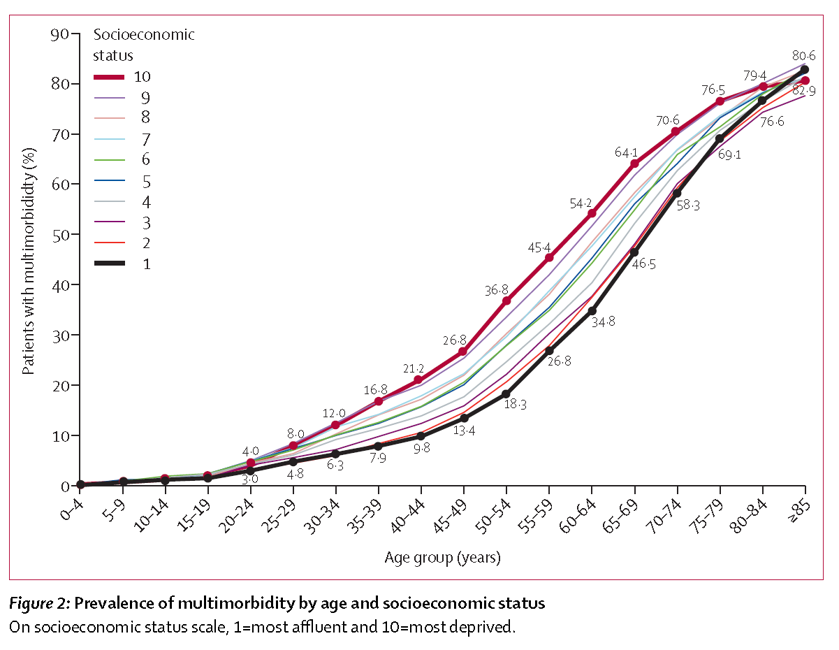
\includegraphics[width=0.8\textwidth, height=0.6\textheight]{images/Prev_multi_morb.png}}
\end{figure}

Barnett et al (2012)

\end{block}

\end{frame}

\begin{frame}{Project outline}

\begin{block}{Background (b) What we know..}

\begin{itemize}
\item<1-> There is a strong socioeconomic gradient observed for those with multimorbidity which feeds the inverse care law in primary care services.
\item<2-> MM associated with higher mortality, psychological distress, worse QOL, worse functional status, and increased health care use.
\item<3-> But what about social care?????
\end{itemize}

\end{block}

\end{frame}

\begin{frame}{Project outline (c) Social Care}

\begin{quote}
``Social care supports people of all ages with certain physical,
cognitive or age-related conditions in carrying out personal care or
domestic routines. It helps people to sustain employment in paid or
unpaid work, education, learning, leisure and other social support
systems. It supports people in building social relationships and
participating fully in society.'' \footnote<.->{Commission on Funding of
  Care and Support. (2011) Fairer Care Funding: The Report of the
  Commission on Funding of Care and Support.}
\end{quote}

Definitional split:-

\begin{itemize}
\tightlist
\item
  Home Care
\item
  Care Home
\item
  Nursing Home
\end{itemize}

\end{frame}

\begin{frame}{Project outline}

\begin{block}{Background (c) Social care and multimorbidity}

\begin{figure}
\centerline{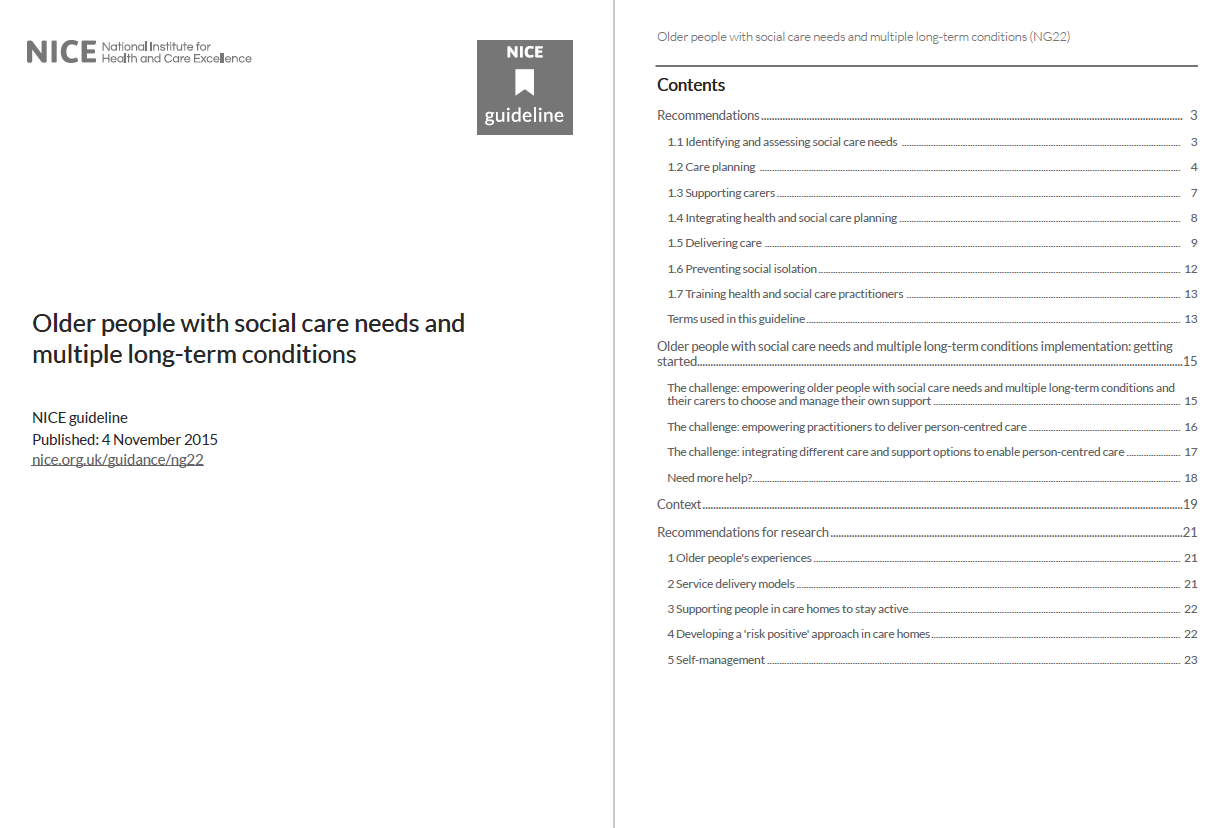
\includegraphics[width=0.8\textwidth, height=0.6\textheight]{images/NICE.png}}
\end{figure}

\end{block}

\end{frame}

\begin{frame}{}

\begin{figure}
\centerline{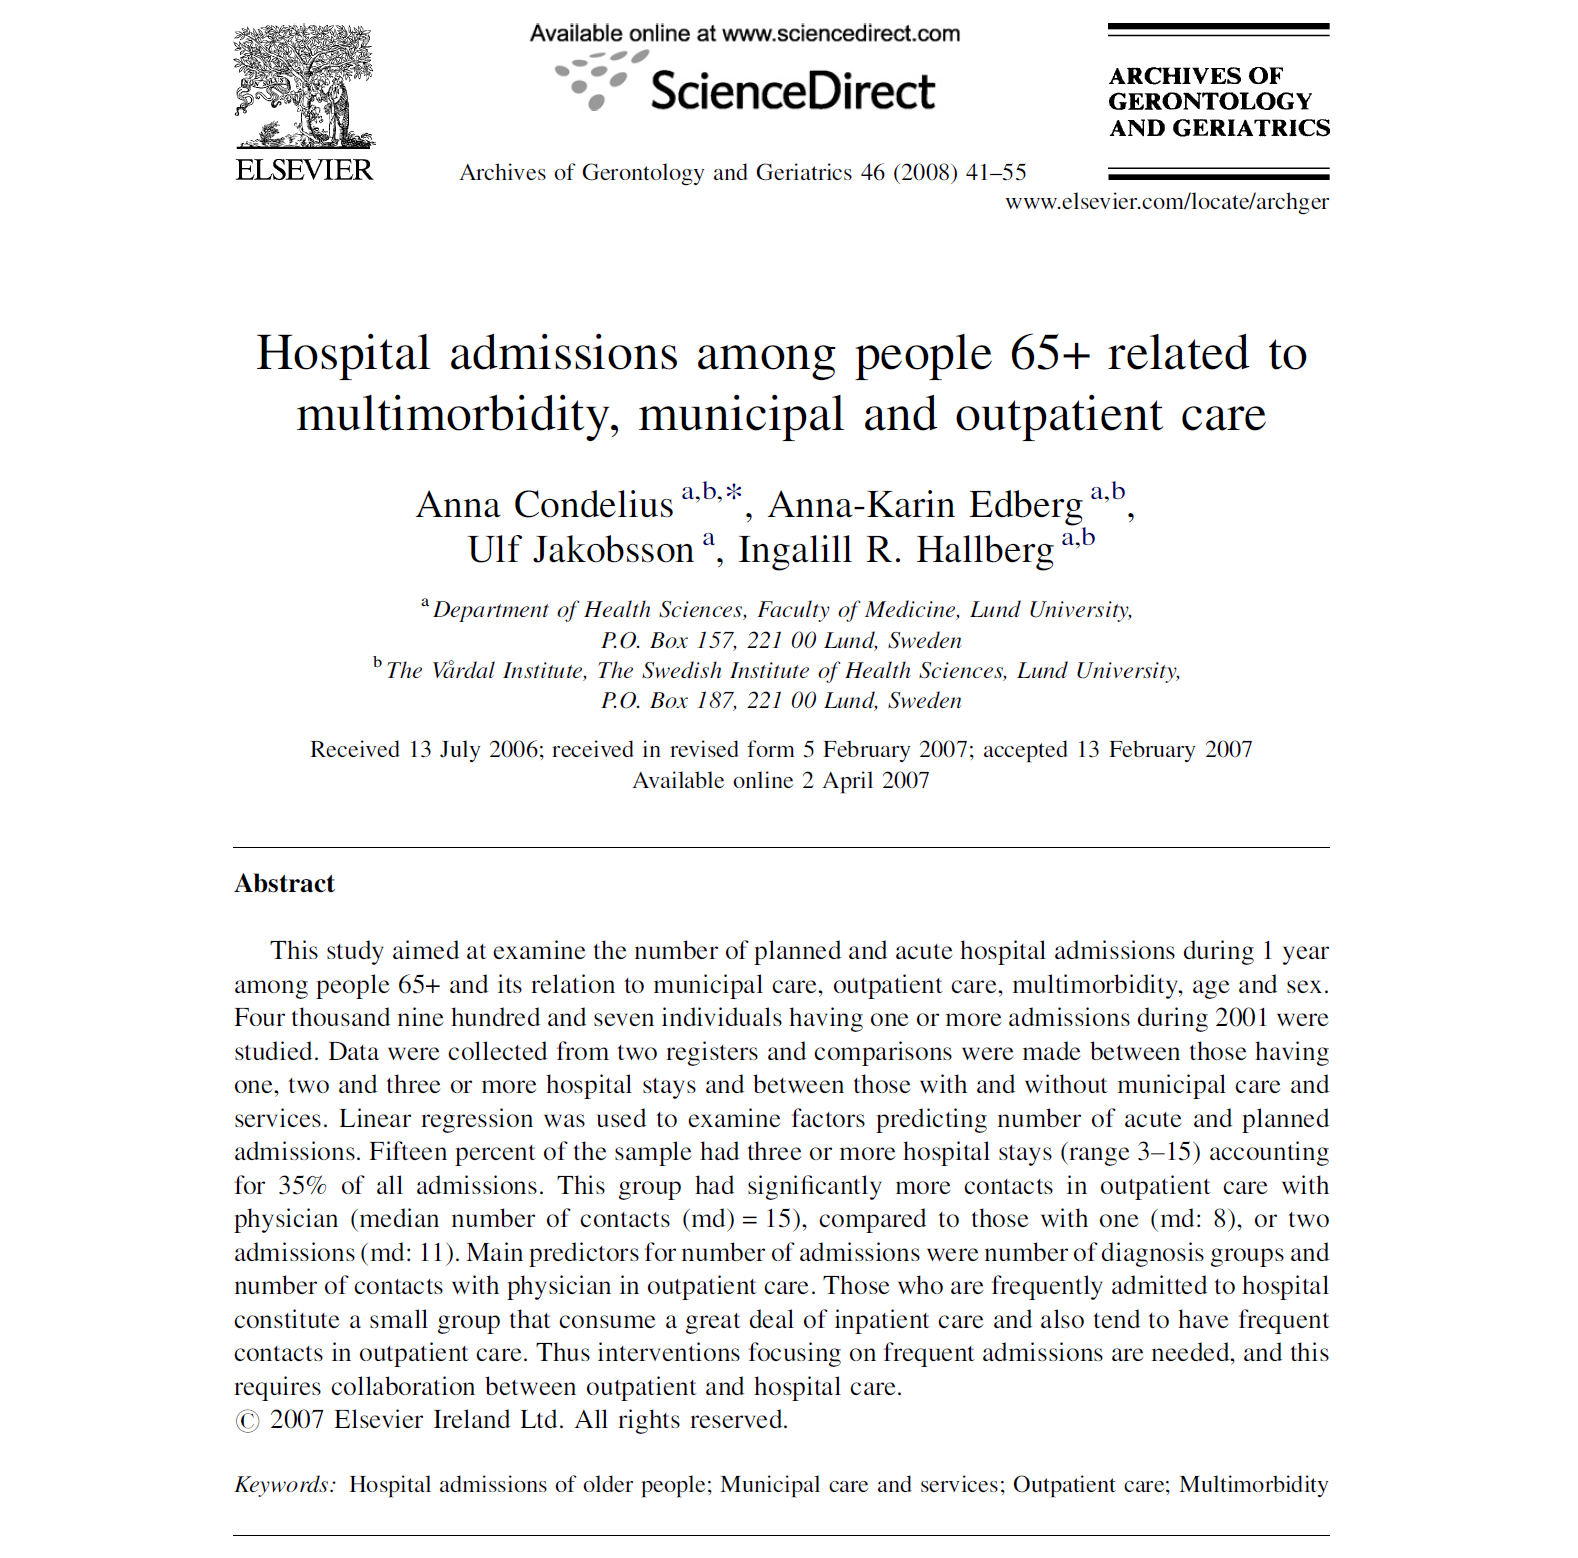
\includegraphics[width=\textwidth,height=0.8\textheight,keepaspectratio]{images/Condelius.PNG}}
\end{figure}

\end{frame}

\begin{frame}{}

\begin{figure}
\centerline{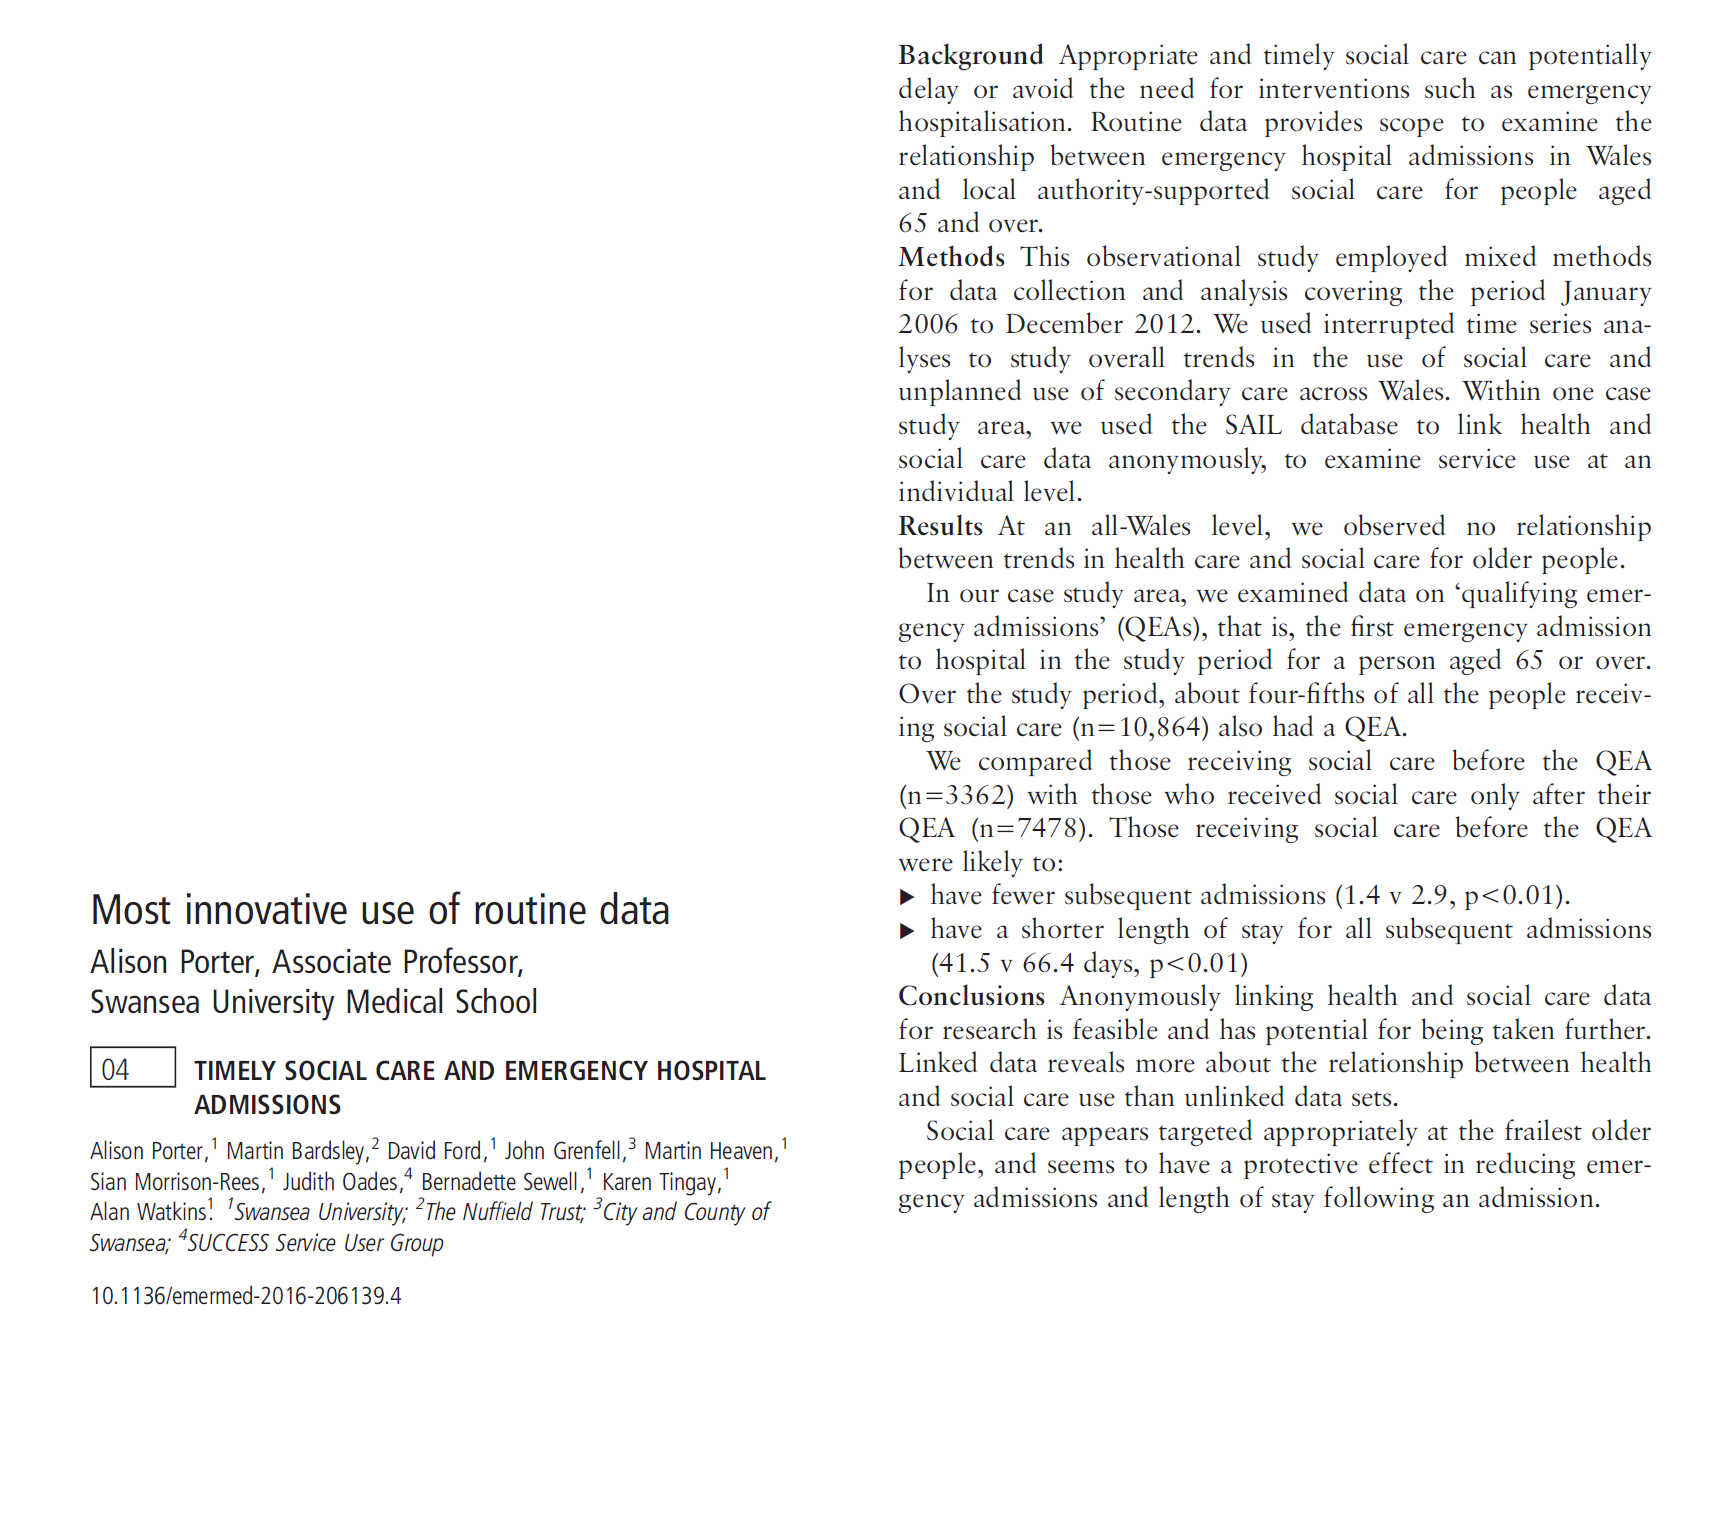
\includegraphics{images/porter.png}}
\end{figure}

\end{frame}

\begin{frame}{Project outline}

\begin{block}{Background (d) Social Care}

\begin{figure}
\centerline{\includegraphics[width=0.8\textwidth, height=0.6\textheight]{images/3MT_plot.png}}
\end{figure}

\faGithub\href{https://github.com/davidhen/social_care_open_data/blob/master/rmds/3MT_plot.Rmd}{ link to code}

\end{block}

\end{frame}

\begin{frame}{Project outline}

\begin{block}{Aims}

\begin{itemize}
\item<1-> Describe and and compare social inequalities in the use of social care services using linked health and social care data. 
\item<2-> Explore the effects of social care use for those with multimorbidity on;
\begin{itemize}
\item unscheduled health care use
\item mortality
\end{itemize}
\item<3-> Assess the validity of existing administrative data on social care for research purposes. 
\end{itemize}

\end{block}

\end{frame}

\begin{frame}{Project outline}

\begin{block}{Research questions:}

In people over the age of 65 in Scotland:

\begin{enumerate}
\item
\begin{enumerate}[(a)]
\item What are the socioeconomic, demographic, and geographic patterns in the use of social care? 
\item Is there an association between multimorbidity status and the amount and type of social care use over time? Does this vary by the patterns described in 1(a)?  
\end{enumerate}
\item 
\begin{enumerate}[(a)]
\item Is there an association in the use of social care services, multimorbidity status and unscheduled health care use?
\item Do multimorbidity status and social care use predict mortality?
\end{enumerate}
\end{enumerate}

\end{block}

\end{frame}

\begin{frame}{Project outline}

\begin{block}{Data sources}

\begin{itemize}
\item<1-> Demographics, Deaths, and SIMD (CHI database and NSS)
\item<1-> Social care survey (Scottish Government)
\item<1-> Prescribing information (ISD)
\item<1-> Unscheduled Care Data Mart (ISD)
\item<1-> SMR01, SMR04, A \& E, and USC LTC diagnoses
\end{itemize}

\end{block}

\begin{block}{Study period}

\begin{itemize}
\item<2-> 1st April 2011 to 31st March 2016
\end{itemize}

\end{block}

\begin{block}{Cohort}

\begin{itemize}
\item<3-> Everyone born before 31st March 1951 (over 65s)
\end{itemize}

\end{block}

\end{frame}

\begin{frame}{Project outline}

\begin{longtable}[]{@{}lll@{}}
\toprule
& n & Total number of records\tabularnewline
\midrule
\endhead
Total Cohort & 1,134,445 &\tabularnewline
Total Deaths & 274,011 &\tabularnewline
At least one prescription & 1,109,168 & 134 million\tabularnewline
Captured by social care survey & 227,345 & 663,809\tabularnewline
At least one episode USC & 845,893 & 3,772,402\tabularnewline
\bottomrule
\end{longtable}

\end{frame}

\begin{frame}{Progress}

\begin{block}{Weekly variation in number of individuals receiving home
care in Renfrewshire council area}

\begin{figure}
\centerline{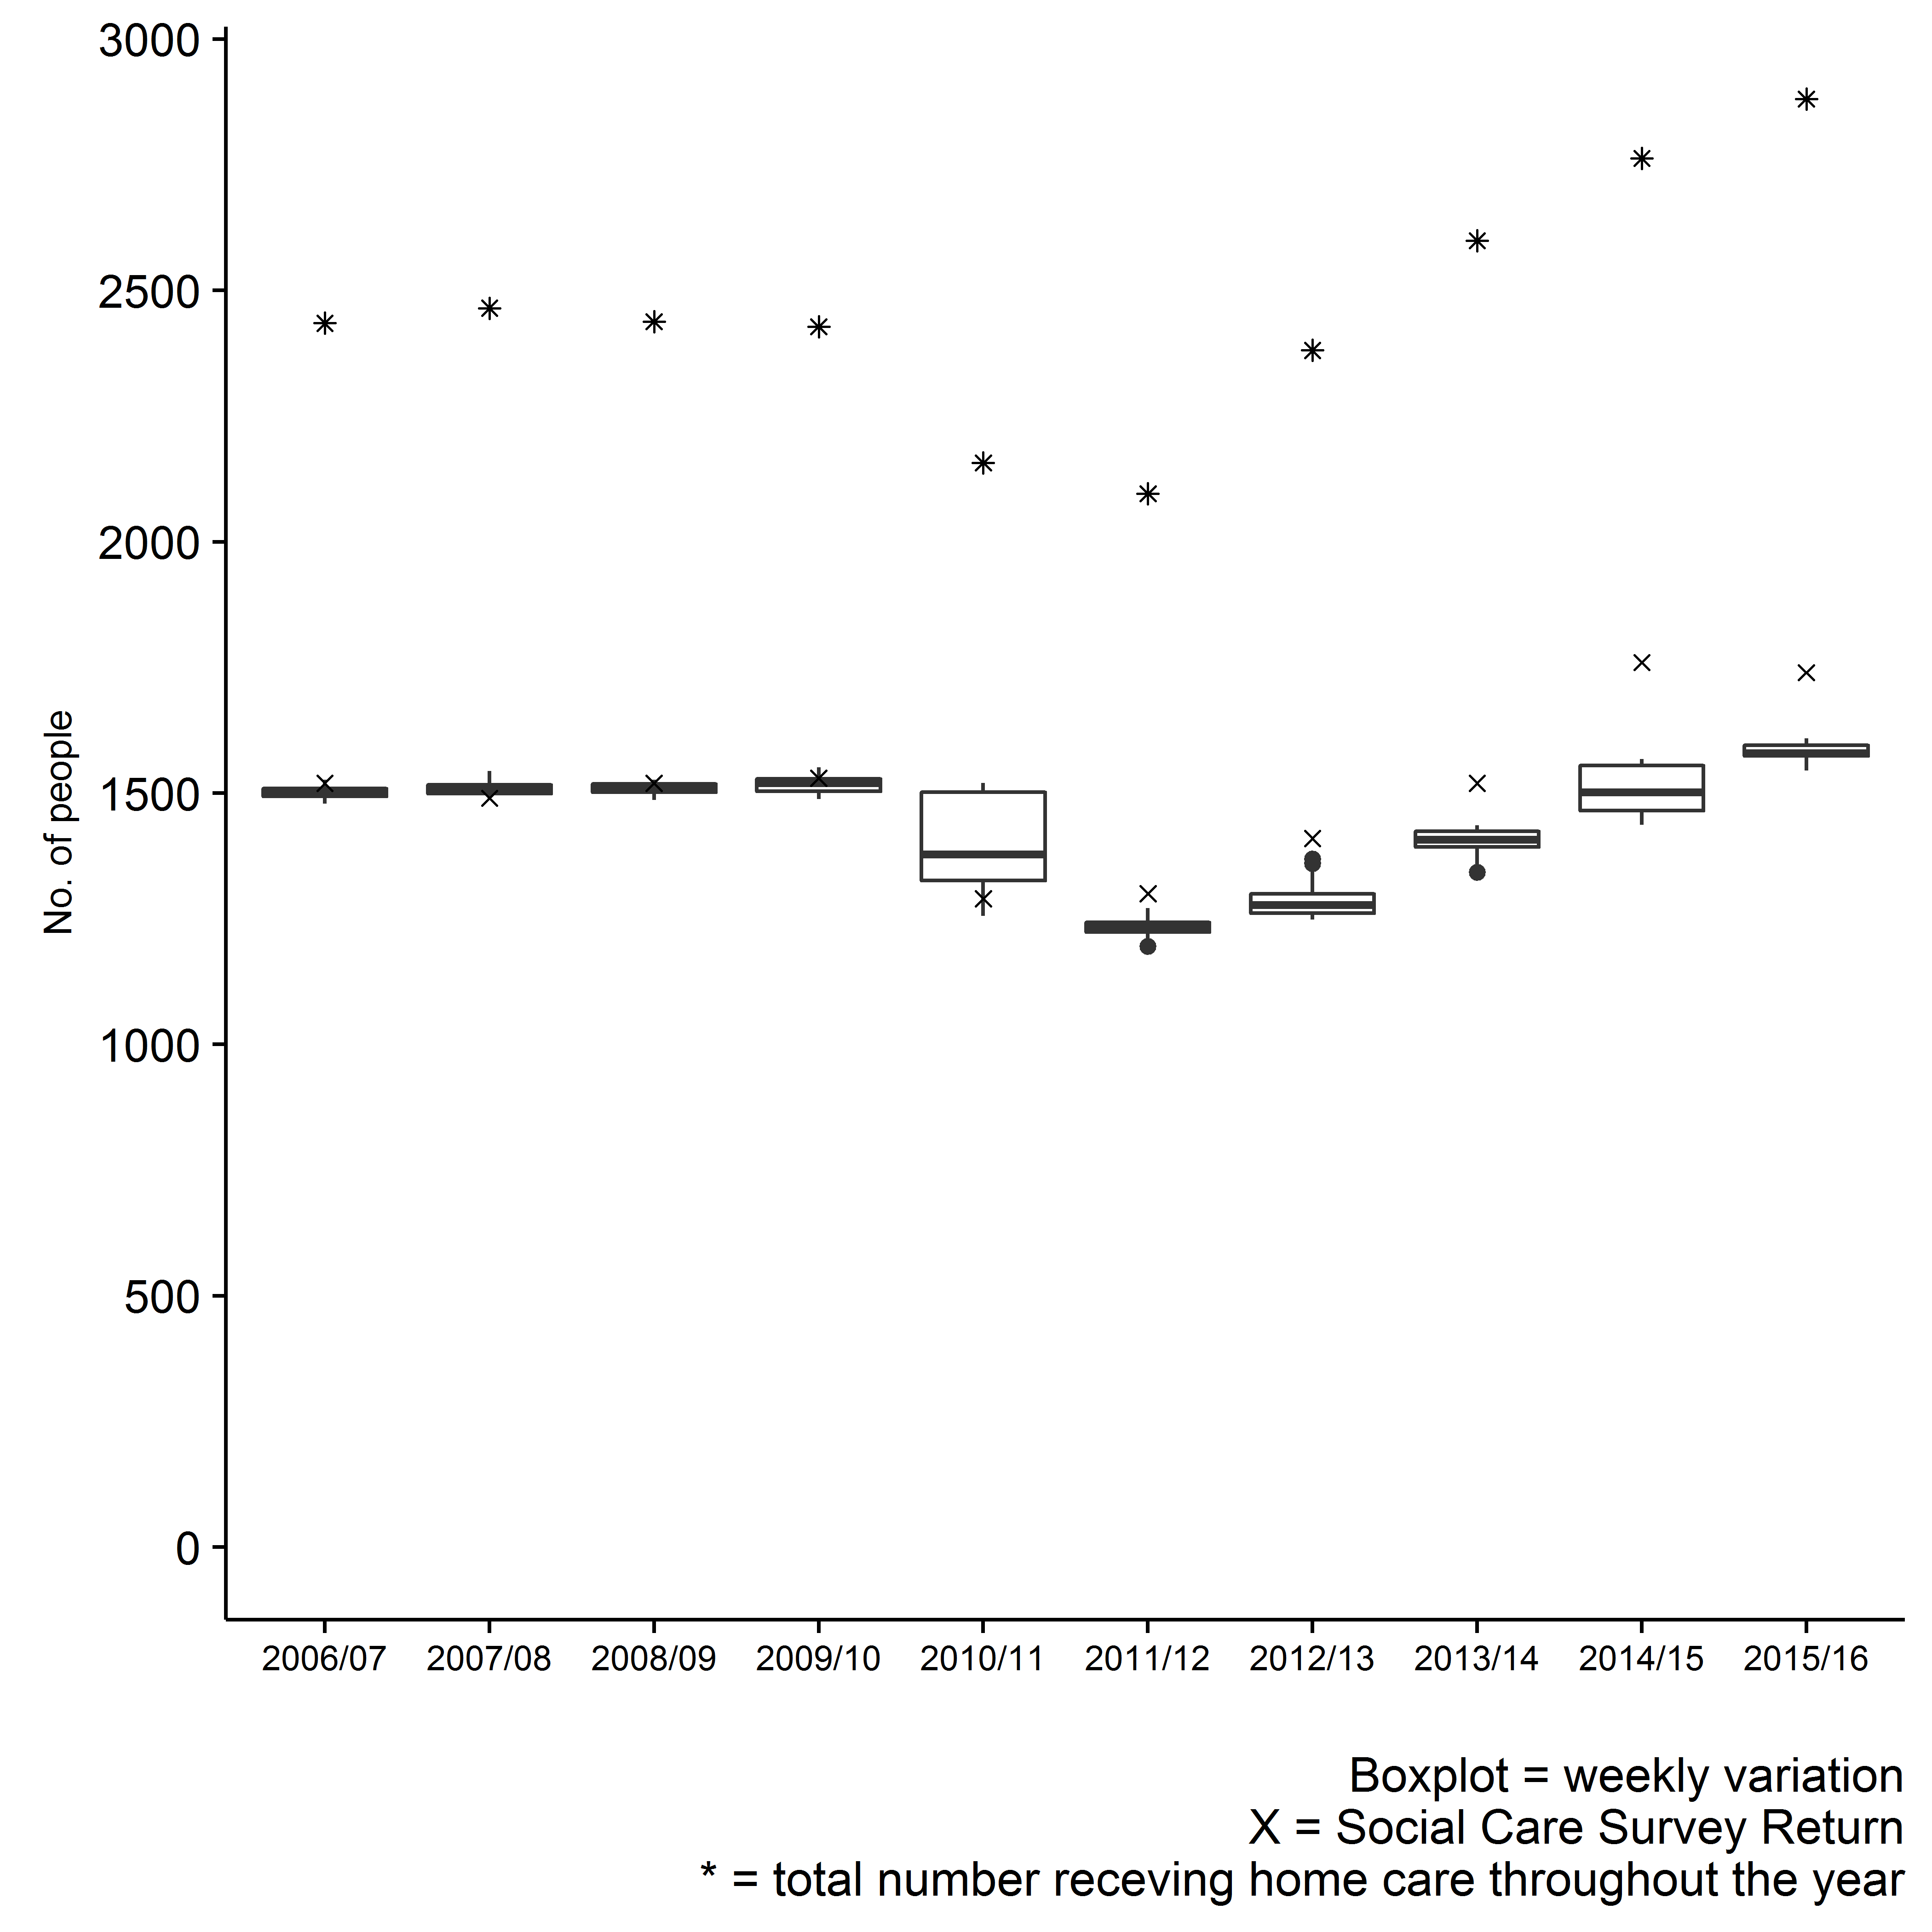
\includegraphics[width=0.8\textwidth, height=0.7\textheight]{images/renfrew.png}}
\end{figure}

\end{block}

\end{frame}

\begin{frame}{Progress}

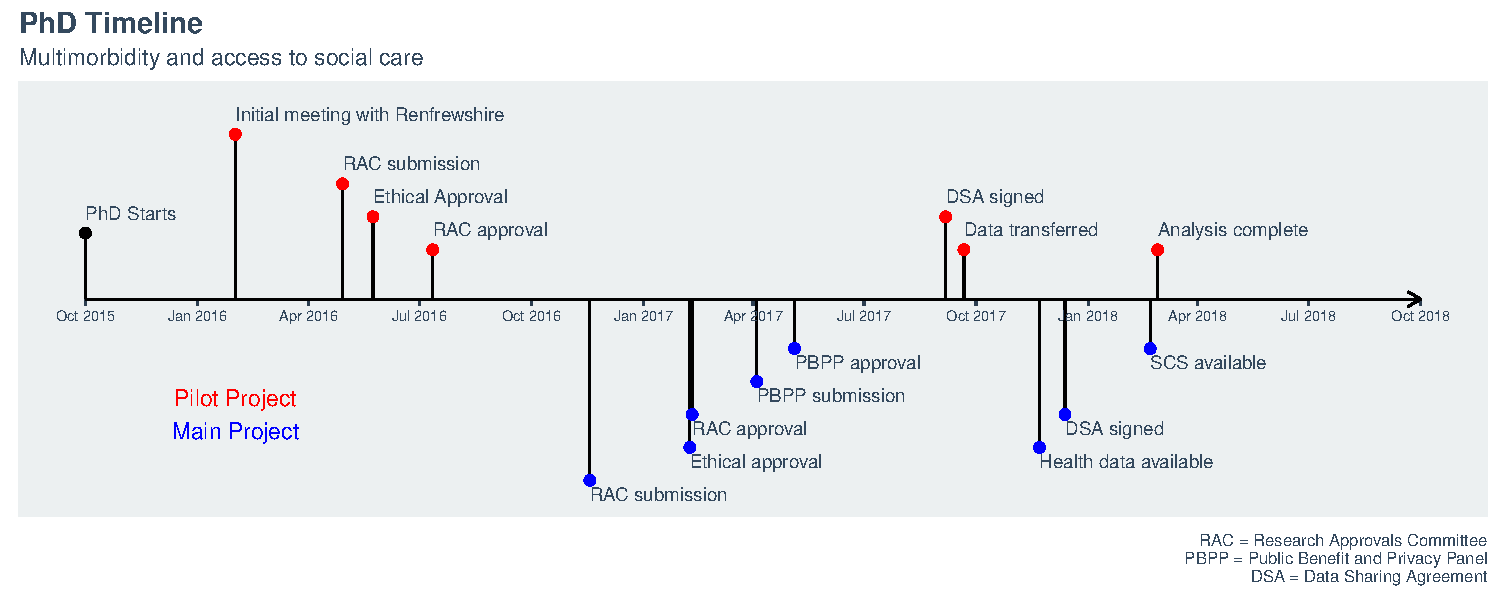
\includegraphics{Farr-2018_files/figure-beamer/timeline-1.pdf}

\end{frame}

\begin{frame}{Any Questions ??}

\begin{figure}
\centerline{
\includegraphics[width=0.8\textwidth, height=0.7\textheight]{images/questions.png}}
\end{figure}

\end{frame}

\end{document}
